\documentclass[12pt%
%,draft%
,aspectratio=169%
]{beamer}
%
\usepackage{fontspec}
\defaultfontfeatures{Ligatures=TeX}
%\setsansfont{Liberation Sans}
\usepackage{polyglossia}
\setdefaultlanguage{ngerman}
% Alternative template for talks of the Freie Universität Berlin.
% Created by Leonard R. König, <leonard.koenig@fu-berlin.de> following the
% guidelines on www.fu-berlin.de/cd
%
% (c) Leonard König, CC BY 4.0
%
% This template was written against UTF-8 capable LaTeX engines, specifically
% LuaLaTeX.

% Trying to get rather close to the ppt/odp template:
%  http://www.fu-berlin.de/sites/cd/downloads_container/PowerPoint_Praesentation_Anleitung.pdf

%%% font styles
\setbeamerfont{frametitle}{series=\bfseries}
\setbeamerfont{footline}{series=\bfseries}
\setbeamerfont{headline}{series=\bfseries}
\setbeamerfont{alerted text}{series=\bfseries}
%%%

% colordefs
\definecolor{fu_darkblue}{RGB}{0,51,102}
\definecolor{fu_seablue}{RGB}{0,102,204}
\definecolor{fu_lightblue}{RGB}{204,214,224}
\definecolor{fu_green}{RGB}{153,204,0}
\definecolor{fu_lightgrey}{RGB}{128,128,128}
\definecolor{fu_grey}{RGB}{95,95,95}
%
\definecolor{fu_red}{RGB}{204, 0, 0} % red text (used by \alert)
%%% end colordefs

%%% colors
\setbeamercolor*{title}{fg=fu_darkblue}
\setbeamercolor*{subtitle}{fg=fu_seablue}
\setbeamercolor*{frametitle}{fg=fu_darkblue}
\setbeamercolor*{footline}{fg=fu_grey,bg=fu_lightblue}
\setbeamercolor*{headline}{fg=fu_grey}

\setbeamercolor*{normal text}{fg=black}
\setbeamercolor*{alerted text}{fg=fu_red}
\setbeamercolor*{example text}{fg=fu_green}
\setbeamercolor*{structure}{fg=fu_darkblue}

\setbeamercolor*{block title}{fg=white,bg=black!50}
\setbeamercolor*{block title alerted}{fg=white,bg=black!50}
\setbeamercolor*{block title example}{fg=white,bg=black!50}

\setbeamercolor*{block body}{bg=black!10}
\setbeamercolor*{block body alerted}{bg=black!10}
\setbeamercolor*{block body example}{bg=black!10}

\setbeamercolor{bibliography entry author}{fg=fu_darkblue}

\setbeamercolor{item}{fg=fu_darkblue}
\setbeamercolor{navigation symbols}{fg=fu_lightgrey,bg=fu_grey}
%%% end colors

%%% title page
% Display logo (if exists) and right next to it, put our title + subtitle
\defbeamertemplate*{title page}{fu_titlepage}
{%
	\hskip .3\textheight
	\begin{minipage}[.4\textheight]{\textwidth}
		\begin{minipage}[.4\textheight]{0.25\textwidth}
			\inserttitlegraphic
		\end{minipage}%
		\begin{minipage}[.4\textheight]{0.75\textwidth}
			\begin{beamercolorbox}{title}
				\usebeamerfont{title}\inserttitle\par%
			\end{beamercolorbox}
			\vfill
			\ifx\insertsubtitle
				\@empty%
			\else
				\begin{beamercolorbox}{subtitle}
					\usebeamerfont{subtitle}\insertsubtitle\par
				\end{beamercolorbox}
			\fi
		\end{minipage}
	\end{minipage}%
	\hskip .3\textheight
}
%%% end title page

%%% headline
% display title, author and institute on the left;
% logo on the right.
\newcommand{\headlinetext}
{%
	\inserttitle\\[0.3em]%
	\insertauthor, %
	\insertshortinstitute
}
\newlength{\headlinewidth}
\setlength{\headlinewidth}{\paperwidth}
\addtolength{\headlinewidth}{-2\marginparsep}
\setbeamertemplate{headline}
{%
	\begin{beamercolorbox}[wd=\paperwidth]{headline}%
		\vskip5pt
		{\hspace*{\marginparsep}}%
		\parbox{.5\headlinewidth}
		{%
			\usebeamertemplate{title in head/foot}%
			\headlinetext%
		}%
		\begin{minipage}{.5\headlinewidth}%
			\hfill\usebeamertemplate*{logo}
		\end{minipage}%
		{\hspace*{\marginparsep}}%
	\end{beamercolorbox}%
}
%%% end headline

%%% footline
% title + date on the left, frame number on the right
\newcommand{\footlinetext}
{%
	\usebeamerfont{shorttitle}\insertshorttitle, %
	\usebeamerfont{shortdate}\insertshortdate
}
\setbeamertemplate{footline}
{%
	\begin{beamercolorbox}{footline}
		\vskip2pt
		\hspace{\marginparsep}%
		\footlinetext\hfill%
		\insertframenumber%
		\hspace{\marginparsep}
		\vskip2pt
	\end{beamercolorbox}%
}
%%% end footline

% don't use default templates for sidebars
\setbeamertemplate{sidebar right}{}
\setbeamertemplate{sidebar left}{}
\setbeamertemplate{title page}[fu_titlepage]
\usepackage{amsmath}
\usepackage{amsfonts}
\usepackage{amssymb}
\usepackage{graphicx}
\usepackage{algorithm}
\usepackage[noend]{algpseudocode}
%\usepackage{algorithmic}
\usepackage{tikz}
\usetikzlibrary{arrows,shapes,automata,petri,positioning,calc}
\usepackage{graphicx}
\usepackage{subfig}
\usepackage{pgfplots}
\usepackage{venndiagram}
\usepackage{ stmaryrd }
\usepackage[normalem]{ulem}
\usepackage{circuitikz}
\usepackage{bohr}
\usepackage{csquotes}

\setbeamercolor{block title}{use=structure,fg=white,bg=structure.fg!75!black}
\setbeamercolor{block body}{parent=normal text,use=block title,bg=block title.bg!10!bg}


\author{Benjamin Tröster}
\title[Zahlendarstellung]{Zahlendarstellung}
%\subtitle[Markov Models]{...}
%\pgfdeclareimage{titlegraphic}{../res/dwarf_logo2.png}
%\titlegraphic{\pgfuseimage{titlegraphic}}
%\date{}
%\subject{}
%
% FU settings
\institute[HTW Berlin]{Hochschule für Technik und Wirtschaft Berlin}
%\pgfdeclareimage[height=0.9cm]{logo}{../res/dwarf_logo}
%\logo{\pgfuseimage{logo}}
%
\usepackage[
backend=biber,
citestyle=alphabetic,bibstyle=authoryear
]{biblatex}
\addbibresource{sources.bib}


\begin{document}

\begin{frame}
\titlepage
\end{frame}

\begin{frame}{Fahrplan}
\tableofcontents[hideothersubsections]
\end{frame}

\section{Einleitung}
\begin{frame}{Heute}
\begin{itemize}
	\item Coronabedingt: Sprung von Schaltkreisen und Transistoren zur Zahlendarstellung
	\item Ziel: Wir bauen ein Rechenwerk (ALU) aus Schaltkreisen mithilfe von Gattern
	\item Zwischenziel: Wie können wir die Zahlen im Rechner darstellen?
	\item Darstellung der natürlichen Zahlen $\mathbb{N} \quad \surd$
\end{itemize}
\end{frame}



\section{Ganzen Zahlen}
\begin{frame}{Die ganzen Zahlen (anschaulich)}
\begin{center}
\Huge{$\ldots, -2, -1, 0,1,2,\ldots$}
\end{center}
\begin{itemize}
	\item kennt (fast) jedes Kind
	\item beginnen nirgends
	\item Es gibt positive und negative Zahlen
	\item Schulden, aber keine Tortenstücke
\end{itemize}
\end{frame}

\begin{frame}{Die ganzen Zahlen (konstruktiv)}
\begin{itemize}
	\item \textcolor{blue}{Problem}
	\begin{itemize}
		\item Ist $n > m$, so hat $x + n = m$ keine Lösung $x \in \mathbb{N}$
	\end{itemize}
	\item \textcolor{blue}{Ausweg}
	\begin{itemize}
		\item Erweitere $\mathbb{N}$ zu $\{x = (n, m)\}$. Wir schreiben $(n, m) = m - n$.
	\end{itemize}
	\item \textcolor{blue}{Neues Problem}
	\begin{itemize}
		\item Nicht eindeutig: $x + 2 = 1$ und $x + 1 = 0$ hätten verschiedene Lösungen!
	\end{itemize}
	\item \textcolor{blue}{Neuer Ausweg}
	\begin{itemize}
		\item Äquivalenzklassen 
	\end{itemize}
\end{itemize}
\end{frame}

\begin{frame}{Anzahl der ganzen Zahlen}
\begin{center}
	Gibt es mehr ganze Zahlen als natürliche Zahlen?
\end{center}
\end{frame}

\begin{frame}{Anzahl der ganzen Zahlen}
\begin{center}
	Gibt es mehr ganze Zahlen als natürliche Zahlen?
	\begin{itemize}
		\item \textcolor{red}{Ja!} -- denn $-1 \in \mathbb{Z}$ aber $-1 \not \in \mathbb{N}$
	\end{itemize}
\end{center}
\end{frame}

\begin{frame}{Anzahl der ganzen Zahlen}
	Gibt es mehr ganze Zahlen als natürliche Zahlen?
	\begin{itemize}
		\item \sout{\textcolor{red}{Ja!} -- denn $-1 \in \mathbb{Z}$ aber $-1 \not \in \mathbb{N}$}
		\item \textcolor{red}{Nein!} -- denn $\mathbb{Z}$ ist abzählbar.
	\end{itemize}
	Es gibt eine bijektive Abbildung $\varphi : \mathbb{N} \to \mathbb{Z}$
\end{frame}

\subsection{Zifferndarstellung}
\begin{frame}{Zifferndarstellung mit Vorzeichenbit}
\begin{itemize}
	\item Darstellung positiver Zahlen
	$$
		(z_k z_{k-1} \ldots z_0)q = \sum_{i = 0}^k z_i q^i \qquad z_i \in \mathcal{Z}= \{0,1, \ldots q-1 \}
	$$
	\item Zusätzliches Symbol: \enquote{$-$}
	\item Darstellung negativer Zahlen
	$$
		(z_k z_{k-1} \ldots z_0)q = \sum_{i = 0}^k z_i q^i \qquad z_i \in \mathcal{Z}= \{0,1, \ldots q-1 \}
	$$
	\item \textcolor{blue}{Technische Realisierung:} Vorzeichenbit
\end{itemize}
\end{frame}

\begin{frame}{Dualdarstellung ganzer Zahlen mit Vorzeichenbit}
$$
	\mathbb{Z} = \{ \ldots , 111_2 , 110_2 , 101_2 , 000_2 , 001_2 , 010_2 , 011_2 , . . . \}
$$
\begin{itemize}
	\item Darstellung
	\begin{itemize}
		\item Eindeutigkeit bei endlich vielen Stellen: 1.Stelle = Vorzeichenbit
	\end{itemize}
	\item Keine eindeutige Darstellung von $0: 0 = 000_2 = 100_2$
	\item Addition natürlicher und ganzer Zahlen grundsätzlich verschieden
\end{itemize}
\end{frame}

\begin{frame}{(Technische Realisierung) Betrag \& Vorzeichen}
Eine Stelle wird als Vorzeichenbit benutzt.\\
\begin{itemize}
	\item MSB = Most Significant Bit
\end{itemize}
Das am weitesten links stehende Bit ist das Vorzeichen
\begin{itemize}
	\item MSB = 0 $\Rightarrow$ positive Zahl
	\item MSB = 1 $\Rightarrow$ negative Zahl
\end{itemize}
Beispiel (hier \texttt{WORD} Size):
\begin{itemize}
	\item $\textcolor{red}{0}001 0010 = +18$
	\item $\textcolor{red}{1}001 0010 = -18$
\end{itemize}
Nachteile:
\begin{itemize}
	\item Bei Addition und Subtraktion müssen die Vorzeichen der Operanden gesondert betrachtet werden.
	\item Es gibt zwei Repräsentationen der Zahl $0$
	\item Mit positivem und mit negativem Vorzeichen
\end{itemize}
\end{frame}

\begin{frame}{Dualdarstellung ganzer Zahlen mit Einerkomplement}
\begin{itemize}
	\item Negative Zahlen werden durch das Invertieren aller Bits gebildet
	\begin{itemize}
		\item Null ist eindeutig darstellbar
		\item Nachteil: Woher weiß ich, ob die Zahl negativ oder positiv ist?
	\end{itemize}
\end{itemize}
\end{frame}



\begin{frame}{Dualdarstellung ganzer Zahlen mit Zweierkomplement}
\begin{itemize}
	\item Grundannahme: Feste Anzahl Stellen N
	\item Kochrezept: Das Zweierkomplement von $n < 0$ erhält man durch:
	\begin{itemize}
		\item Dualdarstellung von $-n$, umklappen aller Bits, 1 addieren
	\end{itemize}
	\item Beispiel:
	\begin{itemize}
		\item Bei $N = 4$ Bits soll $n = -3$ dargestellt werden:
		\item $-3 \qquad \to \qquad -(0011_2) \qquad \to \qquad 1100_2 \qquad \to \qquad 1101_2$
	\end{itemize}
\end{itemize}
\end{frame}

\begin{frame}
	\begin{itemize}
		\item Feste Anzahl Stellen $N$
		\item Größte darstellbare natürliche Zahl wäre $2^N - 1 = 111 \ldots 111_2$
		\item Umklappen aller Bits von $n \leq 0$ entspricht: $(2^N - 1) - n = 1 \ldots 1_2 - n$
		\item Addieren von eins führt zu: $(2^N - 1) - n + 1 = 1 \ldots 1 - n + 1$
	\end{itemize}
\end{frame}

\begin{frame}{Zweierkomplement-Darstellung}
Nachteil:
\begin{itemize}
	\item Unsymmetrischer Zahlenbereich. Die kleinste negative Zahl ist betragsmäßig um 1 größer als die größte positive Zahl
\end{itemize}
Beispiel: 3-Bit-ZK-Zahlen
\begin{figure}
\hspace*{4cm}
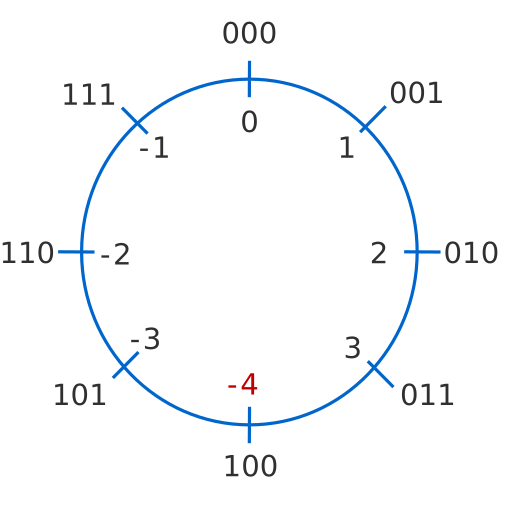
\includegraphics[scale=0.32]{pictures/3bitzk}
\end{figure}

\end{frame}


\begin{frame}{Zweierkomplement-Darstellung}
Nachteil:
\begin{itemize}
	\item Alle anderen negativen Zahlen werden um $1$ verschoben, das \texttt{MSB} bleibt aber gleich $1$
	\item Aus der ersten Stelle kann das Vorzeichen der Zahl abgelesen werden
	\item Aus dieser Konstruktion ergibt sich der Stellenwert des \texttt{MSB} einer Zweierkomplementzahl mit $n+1$ Bit zu $-2^n$:
	$$
		z_n z_{n-1} \ldots z_0 \qquad \text{hat den Wert:}
	$$
	$$
		Z = - (z_n 2^n + z_{n-1} 2^{n-1} + \ldots + z_0)
	$$
\end{itemize}
\end{frame}

\begin{frame}{Darstellung negativer Zahlen -- Beispiel}
Die Zahl $-77_{10}$ soll mit $8$ Bit dargestellt werden
\begin{align*}
	& \quad 77_{10} &= 0100 1101_2 \\
\text{Mit Vorzeichenbit: } & -77_{10} &= 1100 1101_2 \\
\text{Einerkomplement: } & -77_{10} &= 1011 0010_2 \\	
\text{Zweierkomplement: } & -77_{10} &= 1011 0011_2 \\
\end{align*} 
\end{frame}

\begin{frame}{Beispiel Zweierkomplement}
\begin{itemize}
	\item Umrechnung von $-741_{10}$ in dual mithilfe des Zweierkomplements
\end{itemize}
\end{frame}

\begin{frame}{Offset-Dual- (Exzess-)Darstellung}
\begin{itemize}
	\item Wird hauptsächlich bei der Exponenten-Darstellung von Gleitkommazahlen benutzt
	\item Die Darstellung einer Zahl erfolgt in Form ihrer \textcolor{red}{Charakteristik}
	\item Der gesamte Zahlenbereich wird durch Addition einer Konstanten (Exzess, Offset) so nach oben verschoben, dass die kleinste (negative) Zahl die Darstellung $0\ldots 0$ erhält
	\begin{itemize}
		\item Bei $n$ Stellen ist der Offset $2^{n-1}$
		\item Beispiel: $n=8 \Rightarrow$ Offset $128$
	\end{itemize}
	\item Der Zahlenbereich ist hier auch asymmetrisch
\end{itemize}
\end{frame}

\begin{frame}{Zusammenfassung der Möglichkeiten}
\begin{figure}
\center
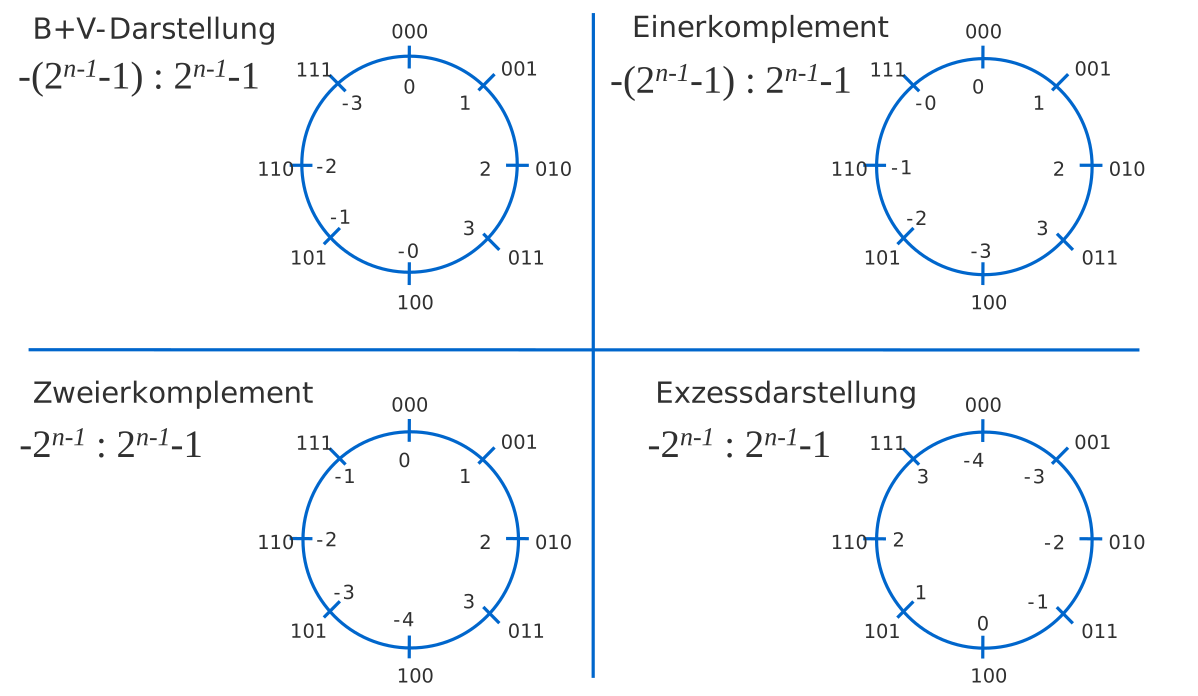
\includegraphics[scale=0.3]{pictures/darstellungen}
\end{figure}
\end{frame}

\begin{frame}{Zusammenfassung der Möglichkeiten}
\begin{table}[]
\begin{tabular}{|c|c|c|c|c|}
\hline
\multicolumn{5}{|c|}{Darstellung mit}                                                                            \\ \hline
\multicolumn{1}{|l|}{Dezimalzahl} & \multicolumn{1}{l|}{B+V} & \multicolumn{1}{l|}{Einer-Komplement} & \multicolumn{1}{l|}{Zweier-Komplement} & Charakteristik \\ \hline
-4 & --- & --- & 100 & 000 \\ \hline
-3 & 111 & 100 & 101 & 001 \\ \hline
-2 & 110 & 101 & 110 & 010 \\ \hline
-1 & 101 & 110 & 111 & 011 \\ \hline
 0 & 100,000 &111, 000 & 000 & 100 \\ \hline
 1 & 001 & 001 & 001 & 101 \\ \hline
 2 & 010 & 010 & 010 & 110 \\ \hline
 3 & 011 & 011 & 011 & 111 \\ \hline
\end{tabular}
\end{table}
\end{frame}


\section*{Quellen}
\appendix
\begin{frame}[allowframebreaks]
  \frametitle<presentation>{Quellen}
\printbibliography
\end{frame}
\end{document}